\documentclass{article}\usepackage{graphicx, color}
%% maxwidth is the original width if it is less than linewidth
%% otherwise use linewidth (to make sure the graphics do not exceed the margin)
\makeatletter
\def\maxwidth{ %
  \ifdim\Gin@nat@width>\linewidth
    \linewidth
  \else
    \Gin@nat@width
  \fi
}
\makeatother

\IfFileExists{upquote.sty}{\usepackage{upquote}}{}
\definecolor{fgcolor}{rgb}{0.2, 0.2, 0.2}
\newcommand{\hlnumber}[1]{\textcolor[rgb]{0,0,0}{#1}}%
\newcommand{\hlfunctioncall}[1]{\textcolor[rgb]{0.501960784313725,0,0.329411764705882}{\textbf{#1}}}%
\newcommand{\hlstring}[1]{\textcolor[rgb]{0.6,0.6,1}{#1}}%
\newcommand{\hlkeyword}[1]{\textcolor[rgb]{0,0,0}{\textbf{#1}}}%
\newcommand{\hlargument}[1]{\textcolor[rgb]{0.690196078431373,0.250980392156863,0.0196078431372549}{#1}}%
\newcommand{\hlcomment}[1]{\textcolor[rgb]{0.180392156862745,0.6,0.341176470588235}{#1}}%
\newcommand{\hlroxygencomment}[1]{\textcolor[rgb]{0.43921568627451,0.47843137254902,0.701960784313725}{#1}}%
\newcommand{\hlformalargs}[1]{\textcolor[rgb]{0.690196078431373,0.250980392156863,0.0196078431372549}{#1}}%
\newcommand{\hleqformalargs}[1]{\textcolor[rgb]{0.690196078431373,0.250980392156863,0.0196078431372549}{#1}}%
\newcommand{\hlassignement}[1]{\textcolor[rgb]{0,0,0}{\textbf{#1}}}%
\newcommand{\hlpackage}[1]{\textcolor[rgb]{0.588235294117647,0.709803921568627,0.145098039215686}{#1}}%
\newcommand{\hlslot}[1]{\textit{#1}}%
\newcommand{\hlsymbol}[1]{\textcolor[rgb]{0,0,0}{#1}}%
\newcommand{\hlprompt}[1]{\textcolor[rgb]{0.2,0.2,0.2}{#1}}%

\usepackage{framed}
\makeatletter
\newenvironment{kframe}{%
 \def\at@end@of@kframe{}%
 \ifinner\ifhmode%
  \def\at@end@of@kframe{\end{minipage}}%
  \begin{minipage}{\columnwidth}%
 \fi\fi%
 \def\FrameCommand##1{\hskip\@totalleftmargin \hskip-\fboxsep
 \colorbox{shadecolor}{##1}\hskip-\fboxsep
     % There is no \\@totalrightmargin, so:
     \hskip-\linewidth \hskip-\@totalleftmargin \hskip\columnwidth}%
 \MakeFramed {\advance\hsize-\width
   \@totalleftmargin\z@ \linewidth\hsize
   \@setminipage}}%
 {\par\unskip\endMakeFramed%
 \at@end@of@kframe}
\makeatother

\definecolor{shadecolor}{rgb}{.97, .97, .97}
\definecolor{messagecolor}{rgb}{0, 0, 0}
\definecolor{warningcolor}{rgb}{1, 0, 1}
\definecolor{errorcolor}{rgb}{1, 0, 0}
\newenvironment{knitrout}{}{} % an empty environment to be redefined in TeX

\usepackage{alltt}
\usepackage{url}
\usepackage{graphicx}
\usepackage{caption}
\usepackage{enumerate}
\usepackage{float}
\title{Global Temperature Anomalies}
\author{Geoffrey Thompson and Sam Benidt}
\date{12/14/2012}
\begin{document}


\maketitle




\begin{figure}[H]
\begin{knitrout}
\definecolor{shadecolor}{rgb}{0.969, 0.969, 0.969}\color{fgcolor}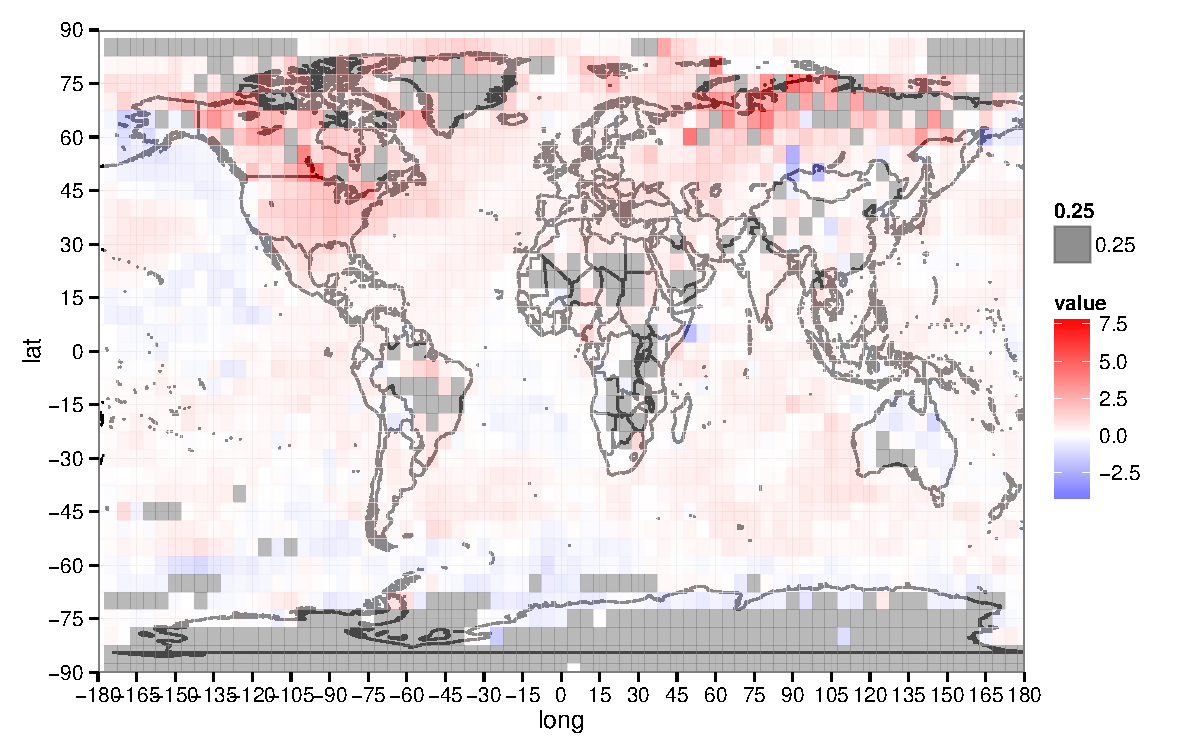
\includegraphics[width=\linewidth]{figure/recent-map} 
\end{knitrout}

\caption{\label{sep2012map}Map of temperature anomalies for September 2012}
\end{figure}

\section{Introduction}

The consensus of climate scientists is that the world has been warming since the Industrial Revolution and that it has been warming faster over the last several decades. This warming is not uniform - the poles are in general are warming much faster than the tropics. The rate of warming has also not been been increasing at a uniform rate over time. For example, the twenty year periods from 1925-1944 and from 1978-1997 have seen the largest increases in temperature throughout the period of the twentieth century. We will be analyzing the HADCRUT4 temperature dataset which has a monthly record of temperature anomalies from a respective 1960-1991 baseline on a $5^{\circ}$ by $5^{\circ}$ gridded basis going back to 1850.  Using this dataset we will graphically explore when and where temperatures have been changing and by how much over the past 162 years. The HADCRUT4 dataset was the subject of some controversy in October when a journalist claimed the data showed no increase in temperature over the last 16 years (1997-2012). We will also attempt to graphically look further into this claim.

\section{Description of Data and Source:}
We pulled data on temperature deviations from the overall 1961 to 1990 temperature trend for each temperature station from the HADCRUT4 near surface temperature data set found at: \url{http://www.metoffice.gov.uk/hadobs/hadcrut4/data/current/download.html}.\\ This data is hosted by the Met Office Hadley Centre. The HADCRUT4 dataset combines data from the  CRUTEM4 and HadSST3 which contain data based on surface air temperature and sea-surface temperature respectively. The data is reported in 100 ensembles. We chose to look at the first ensemble dataset, which was a choice on convenience due to the large nature of each individual ensemble dataset. However, we hope that the same type of analysis recorded here could be used and would be applicable on any of the 100 ensembles.  The Global temperature trend was also downloaded which is computed from average of the trends for the Northern and Southern Hemisphere ((NH +SH)/2).

\section{Data Cleaning/Formatting:}
The temperature deviation data for ensemble 1 was downloaded in a spaced delimited ASCII file.  The ASCII file was opened up in Microsoft Excel and parsed to create a CSV file that contained meta data for the first month of 1850 on the first row, followed by 36 rows and 72 columns of temperature deviations where the entry in row i and column j represented a measurement of temperature deviation for each latitude and longitude. This was followed by another row of metadata describing the second month of 1850 followed by the same 36 rows by 72 columns of temperature deviations and so on for each month. The CSV file was read into R. Each 37th row was deleted (including the first row) since those rows contained meta data. The variables time (in months since 1850), xloc, months (month of year), year(years since 1850). The data were reshaped to using the melt function keeping the variables time, xloc, months, year, and temp, allowing the yloc variable to be formed.  The variables real year and latitude and longitude were introduced to the data set through an appropriate transformation of the variables $year$, $xloc$, and $yloc$. Finally, we able to transform the year and month variables into actual dates using the lubridate package. Global montly temperature deviation data was downloaded as well. However, there was not much work needed to put the data into a useable format besided using the lubridate package again to transform the date variables.

\section{Main Section:}
\subsection*{Increased World Coverage}
The data are a worldwide data set spanning from 1850 to the present, but large portions of the world were still unexplored. The first explorer only set foot on Antarctica in 1840 (or 1821, depending on which account you believe) and reached the south pole in 1911. Whether or not a spot has a set of temperature records in a given year indicates whether scientific meteorology has made it there. In 1850, the records were spotty except in Europe and on the seas.
\begin{figure}
\begin{knitrout}
\definecolor{shadecolor}{rgb}{0.969, 0.969, 0.969}\color{fgcolor}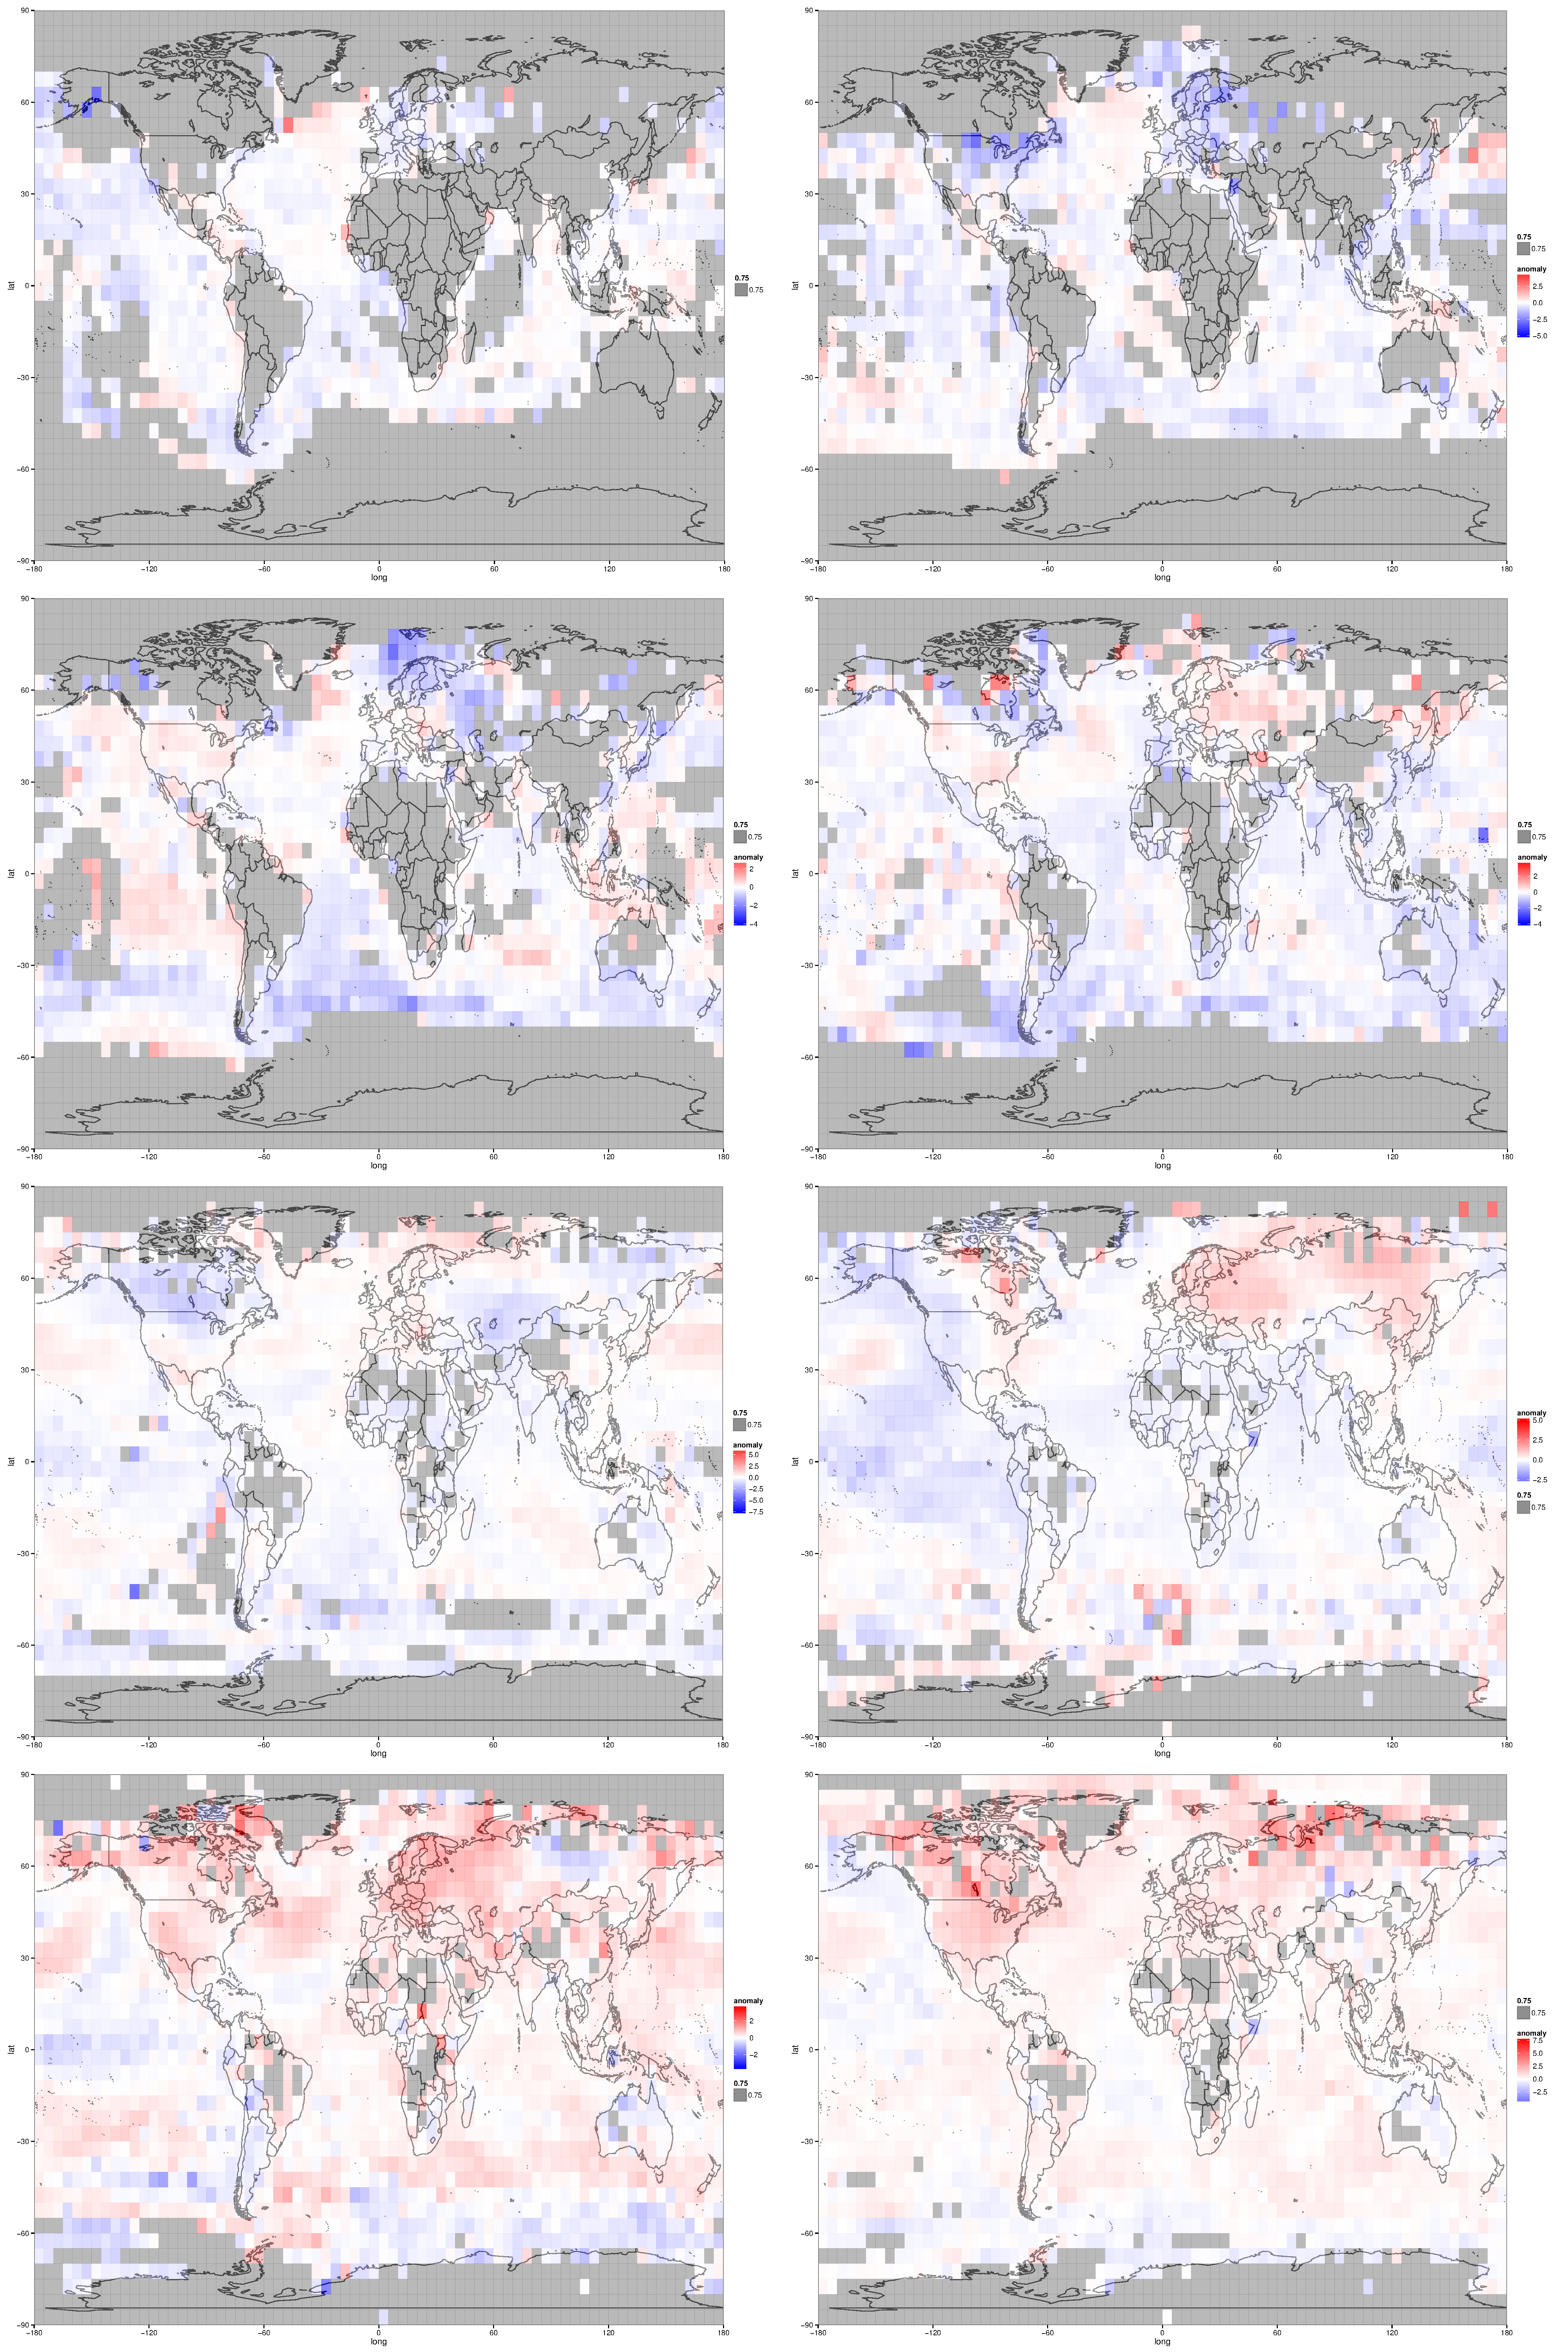
\includegraphics[width=\textwidth,height=.8\textheight]{figure/chunk2} 
\end{knitrout}

\caption{\label{multiyearmap}Maps of temperature anomalies for 1850-2012}
\end{figure}

However, as time passes, the interior of the continents are filled in more until 2012, when only the most remote and uninhabitable areas are neglected, such as the Sahara and the polar regions.

\subsection*{Anomalies vs. Absolute Temperature}
The data presented here are recorded with respect to the 1961-1990 period.  The 1961-1990 period was chosen by the researchers who created this data set since it has some of most consistent data in terms of complete coverage of temperature values. For each station used, the baseline average over 1961-1990 was computed in order to record temperature anomalies by that station per month.

Using temperature anomalies instead of absolute temperatures were useful is solving a few issues of comparability between stations:
\begin{enumerate}
\item Different stations are in different locations (temperature varies by location)
\item Different stations use different recording methods (land vs. sea stations)
\item Different countries use different methods of calculating average monthly temperature
\end{enumerate}
Taken together, using temperature anomalies allows for better comparability between the locations and should resolve some issues in bias when stations use different recording methods.

\subsection*{Global Trends}

The graph below gives the overall deviation in degrees from the 1961 to 1990 trend line by month. Points plotted below zero represent an average temperature in that month below the 1961 to 1990 average and points plotted above zero represents an average temperature above the 30-year average. As can be seen, the vast majority of months from 1850 to 1950 have negative deviations indicating that temperatures from that time period were slightly cooler than the average of temperatures from 1961 to 1990. Starting around the 1970's to 1980's most of the anomalies start to increase such that by 2010 the temperature anomoly is hoving at about 0.5 degrees above the 1961 to 1990 trend line. It can be noted on the graph that there have been two significant warming periods in the 20th century. The periods from 1925 to 1944 and from 1978 to 1997 exhibited some of the largest warming patterns over the past century.
\begin{figure}[H]
\begin{knitrout}
\definecolor{shadecolor}{rgb}{0.969, 0.969, 0.969}\color{fgcolor}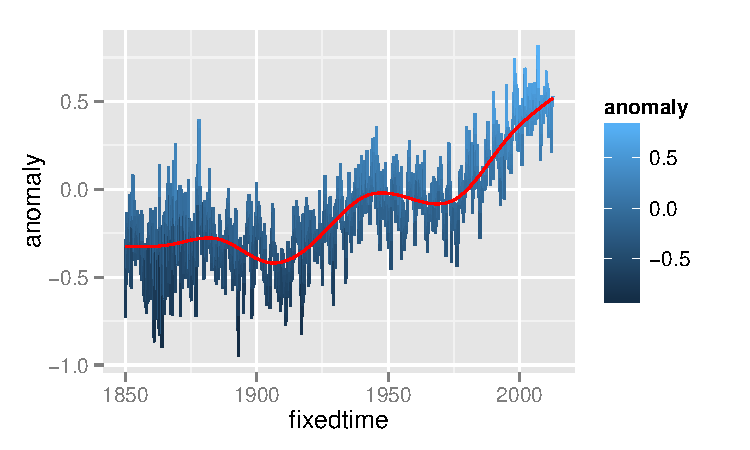
\includegraphics[width=\linewidth]{figure/plot-trend} 
\end{knitrout}

\caption{\label{alltopresent}Time series of global temperature anomalies 1850-present}
\end{figure}
In October of this year, \emph{The Daily Mail} published an article pointing to this data set and saying that there has been no warming in the last 16 years. The graph is roughly reproduced here with a linear trend line drawn - the trend is indeed not significantly different from zero. Some skeptics have pointed to this stagnant trend of no large temperature increase as evidence that we should not worry about the effects of climate change.  \begin{figure}[H]
\begin{knitrout}
\definecolor{shadecolor}{rgb}{0.969, 0.969, 0.969}\color{fgcolor}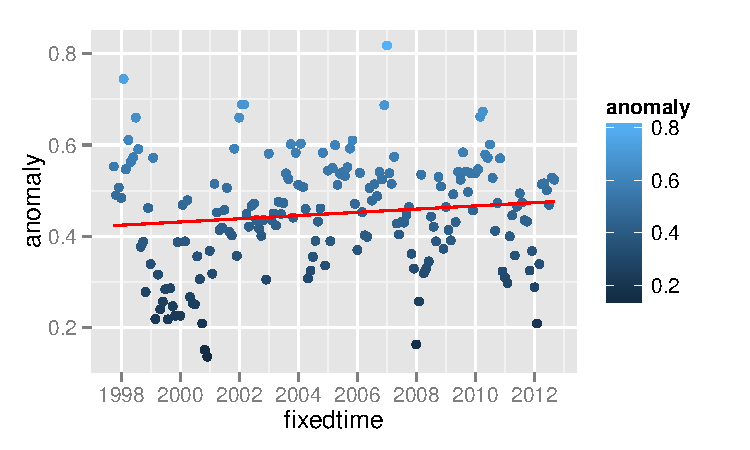
\includegraphics[width=\linewidth]{figure/15-years} 
\end{knitrout}

\caption{\label{last16}Time series of temperature anomalies for last 16 years}
\end{figure}
However, recall Figure 3: this is a time series with quite a lot of variation and a small trend. There are several places in the last 40 years where a flat "trend" could be drawn. The newspaper has also chosen a particularly good point to start from. If we were to extend the range back to 1975, we would see a much different picture of warming trends. Figure 4, with the two trends split up, shows what the choice of starting points in the Daily Mail's article implies about the trend. Without doing any formal hypothesis testing, it looks as if an extremely high outlier in 1997 and a couple relatively lackluster years in the 2000s compared to that outlier have combined to give the appearance of stagnation if you "cherrypick" the starting points of the data.

\begin{figure}[H]
\begin{knitrout}
\definecolor{shadecolor}{rgb}{0.969, 0.969, 0.969}\color{fgcolor}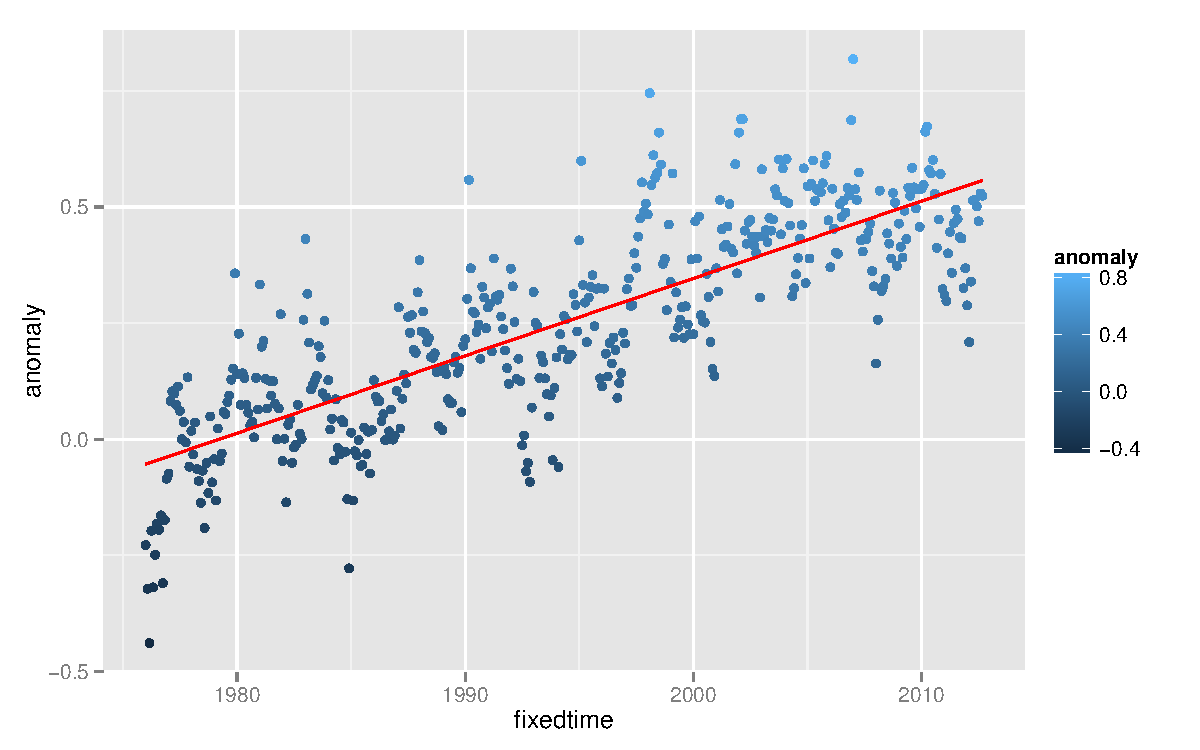
\includegraphics[width=\linewidth]{figure/recent-trend} 
\end{knitrout}

\caption{\label{1975topresent}Time series of temperature anomalies for 1975 to present}
\end{figure}

\subsection*{Locations of Interest}

After looking at global temperature trends, we decided it would be interesting to check out trends in certain locations of interest. As such, we decided to look into the temperature data for Story County, Iowa.

When looking at individual locations, the range of anomalies is much higher than that of the global anomoly graph. Almost all of the anomolies for the global anomoly graphs posted above fell within one degree Celcius of the 1960-1991 trend. Whereas, for Story county, the majority of anomolies fall within 10 degrees Celsius of it's own 1960-1991 trend. We see from the smoothed line that the trend of anomolies has been increasing over time, indicating that Story County has risen in temperature over the past century and a half. Starting in 1850, Story County was about 1 degree Celsius below the 1960-1991 trend while now it is about 1 degree Celsius above the trend.

%Latitude and longitude for story county is at 42.0242? N, 93.5287? W
% This is lat=40 and long=-95 in our dataset
%Latitude and longitude for Augsburg Germany is 48.3647? N, 10.8953? E
% closest is lat=50 and long=10

\begin{figure}[H]
\begin{knitrout}
\definecolor{shadecolor}{rgb}{0.969, 0.969, 0.969}\color{fgcolor}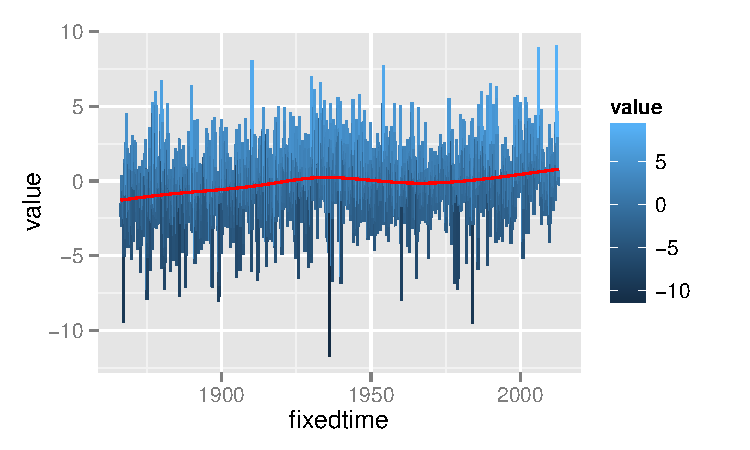
\includegraphics[width=\linewidth]{figure/story-trend} 
\end{knitrout}

\caption{\label{storycount}Time series of temperature anomalies for Story County, IA}
\end{figure}

The trend for Augsburg, Germany is also increasing over time. However, as compared to Story County, Augsburg has had more months with large negative anomalies as compared to large positive anomalies. Again we see that in 1850, Augsburg was about 1 degree Celsius below the 1960-1991 trend while now it is about 1 degree Celsius above the trend. This is similar to where Story County sits at.
\begin{figure}[H]
\begin{knitrout}
\definecolor{shadecolor}{rgb}{0.969, 0.969, 0.969}\color{fgcolor}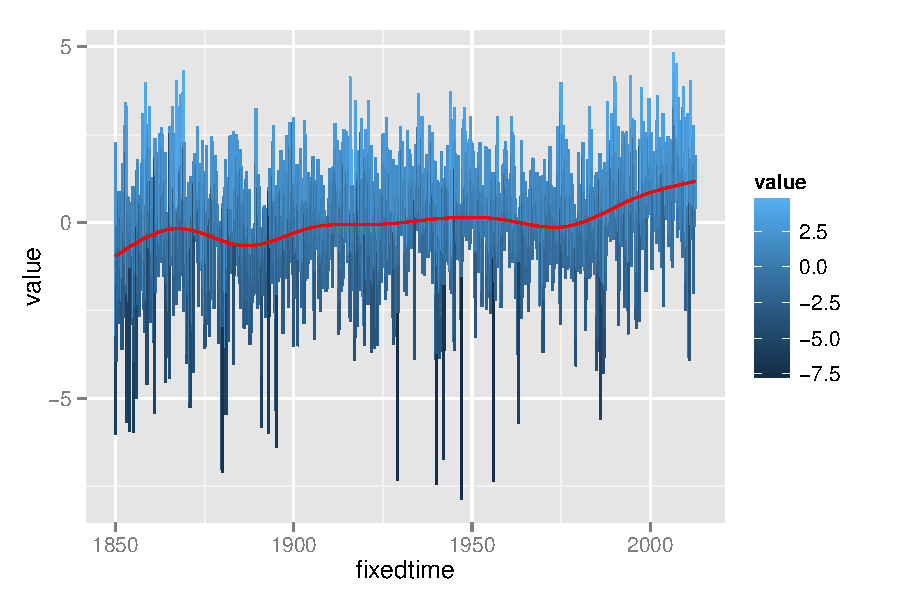
\includegraphics[width=\linewidth]{figure/augsburg-trend} 
\end{knitrout}

\caption{\label{augsburg}Time series of temperature anomalies for Augsburg, Germany.}
\end{figure}

%Chose point in Antartica that actually had data values lat==-75 & long==15

To look at the polar regions, we choose a point with a latitude of 75 degrees South and 15 degrees East. Again, the polor region here is experiencing a warming trend. There is less data available for this location in Antarctica with anomalies only reported back to 1960. As such, we do not know how the temperature trend looks back in the 1800's. However, given the shorter period time as compared to the other graphs for Augsburg and Story County, we still see a significant increasing temperature pattern in this Antarctic location. 

\begin{figure}[H]
\begin{knitrout}
\definecolor{shadecolor}{rgb}{0.969, 0.969, 0.969}\color{fgcolor}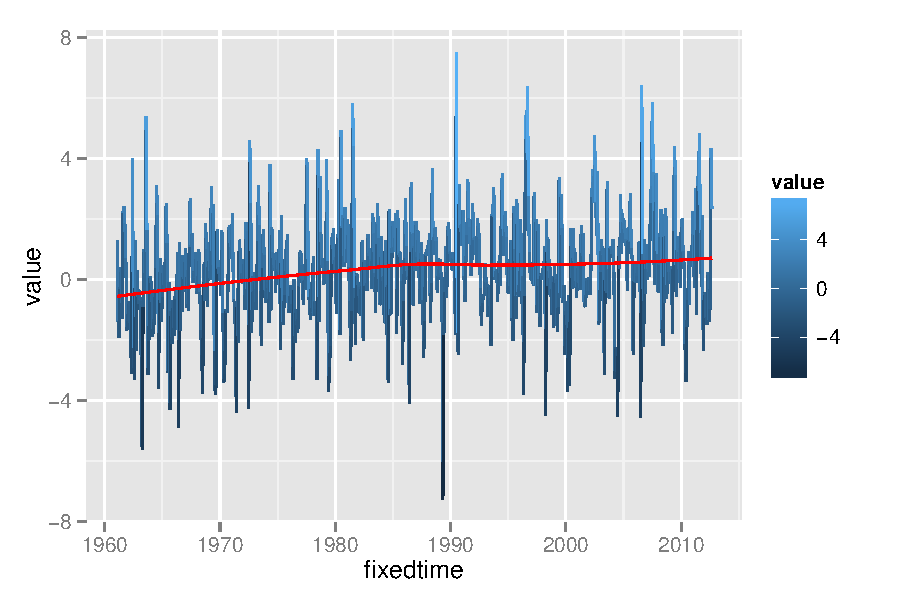
\includegraphics[width=\linewidth]{figure/antartic-trend} 
\end{knitrout}

\caption{\label{antarctica}Time series of temperature anomalies for a station in Antarctica, 1960-present.}
\end{figure}

\subsection{World Maps from 1978 and 1997}

Next, we turn back to some interesting maps of the world colored by anomaly. An interesting comparison in time is between 1978 and 1997 which marked the beginning and conclusion of a substantial warming period during the twentient century. As can be noted in the 1978 map, a significantly larger portion of the map is shaded in blue, while in the 1997 those blue areas change to a neutral white. Further, a lot of areas colored in white in 1978 and colored in red in 1997 and those colored in red in 1978 are a darker shade of red in 1997. These maps show that overall temperatures have risen between 1978 and 1997, regardless of location.

\begin{figure}[H]
\begin{knitrout}
\definecolor{shadecolor}{rgb}{0.969, 0.969, 0.969}\color{fgcolor}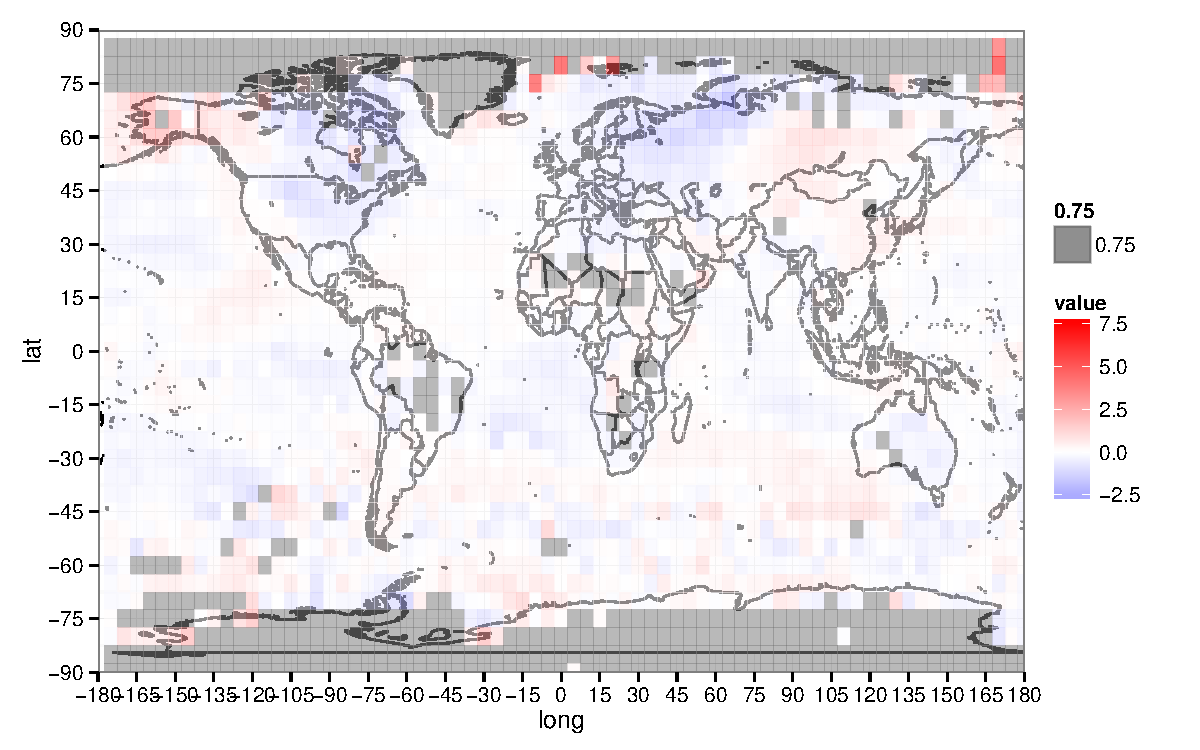
\includegraphics[width=\linewidth]{figure/1978-map} 
\end{knitrout}

\caption{\label{1978map}Map of temperature anomalies for 1978}
\end{figure}

\begin{figure}[H]
\begin{knitrout}
\definecolor{shadecolor}{rgb}{0.969, 0.969, 0.969}\color{fgcolor}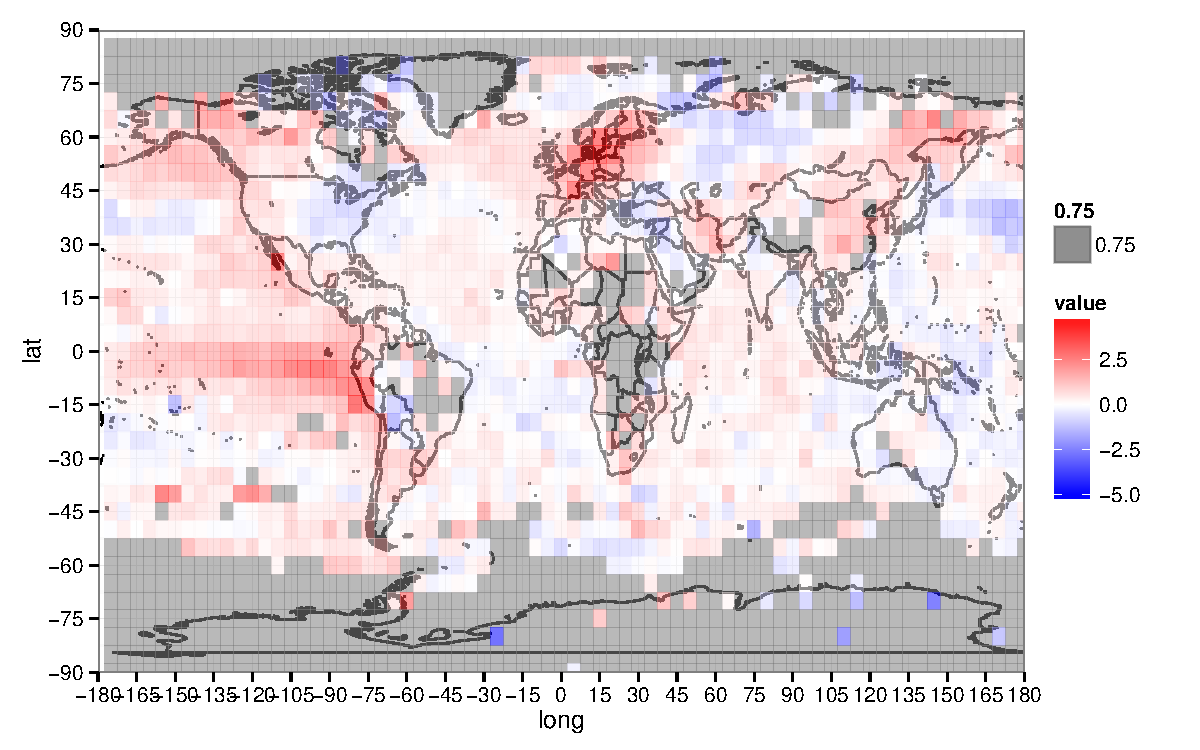
\includegraphics[width=\linewidth]{figure/second1997map} 
\end{knitrout}

\caption{\label{another1997map}Map of temperature anomalies for Summer 1997}
\end{figure}

\section{Conclusion:}
We set out to explore global temperature anomalies graphically over the past century and a half graphically and found some interesting trends. Overall, global temperatures are rising, regardless of location, with 1925-1944 and 1978-1997 showing rapid increases in overall temperature. If you only look locally at the last several years, it is hard to see any trend, but in the larger context it cannot be concluded that the trend has changed.

\section{References}
Morice, C. P., J. J. Kennedy, N. A. Rayner, and P. D. Jones (2012), Quantifying uncertainties in global and regional temperature change using an ensemble of observational estimates: The HadCRUT4 dataset, J. Geophys. Res., 117, D08101, doi:10.1029/2011JD017187.

Rose,D. (2012, October 16). Global warming stopped 16 years ago. \emph{The Daily Mail.} Retrieved 12/10/2012. from \url{http://www.dailymail.co.uk/sciencetech/article-2217286/Global-warming-stopped-16-years-ago-reveals-Met-Office-report-quietly-released--chart-prove-it.html}
\end{document}
